\documentclass[draft]{agujournal2018}
\journalname{JGR: Earth Surface}

\usepackage{apacite}
\usepackage{amsmath,amssymb,amsfonts,amsthm}
\usepackage{comment}
\usepackage{wrapfig}
\usepackage{lipsum}
\usepackage{booktabs} % for wrapping text around tabulars in 
\usepackage{ragged2e}
\usepackage{lineno}
\justifying
\linenumbers


% there is a bug with align environments in conjunction with lineno
% the patch is 
\newcommand*\patchAmsMathEnvironmentForLineno[1]{%
	\expandafter\let\csname old#1\expandafter\endcsname\csname #1\endcsname
	\expandafter\let\csname oldend#1\expandafter\endcsname\csname end#1\endcsname
	\renewenvironment{#1}%
	{\linenomath\csname old#1\endcsname}%
	{\csname oldend#1\endcsname\endlinenomath}}% 
\newcommand*\patchBothAmsMathEnvironmentsForLineno[1]{%
	\patchAmsMathEnvironmentForLineno{#1}%
	\patchAmsMathEnvironmentForLineno{#1*}}%
\AtBeginDocument{%
	\patchBothAmsMathEnvironmentsForLineno{equation}%
	\patchBothAmsMathEnvironmentsForLineno{align}%
	\patchBothAmsMathEnvironmentsForLineno{flalign}%
	\patchBothAmsMathEnvironmentsForLineno{alignat}%
	\patchBothAmsMathEnvironmentsForLineno{gather}%
	\patchBothAmsMathEnvironmentsForLineno{multline}%
}
% from https://tex.stackexchange.com/questions/43648/why-doesnt-lineno-number-a-paragraph-when-it-is-followed-by-an-align-equation?noredirect=1&lq=1


\begin{document}

\title{Joint stochastic model of bedload transport and bed elevations: derivation of heavy-tailed resting times}
\authors{James K. Pierce\affil{1}\thanks{Vancouver, British Columbia, Canada}, and Marwan A. Hassan\affil{1}}
\affiliation{1}{Department of Geography, University of British Columbia}
\correspondingauthor{James K. Pierce}{kpierce@alumni.ubc.ca}

\begin{keypoints}
\item We model fluvial bedload activity and local bed elevation as a two-species stochastic birth-death process.
\item Computations show heavy-tailed power-law distributions of resting times for sediment undergoing burial with tail parameter $\alpha\approx 1.18$.
\item We discuss implications for bedload diffusion and propose a new modeling framework for fluvial morphodynamics.

\end{keypoints}

\begin{abstract}
We present a model of bedload transport and bed elevation changes as a joint stochastic process and use it to obtain resting time distributions for sediment undergoing burial.
Our model predicts heavy-tailed power-law distributions of resting times with tail behavior completely characterized by the mean erosion rate and its scaling with bed elevation changes.
Resting time distributions of sediment undergoing burial are remarkably independent of bedload fluctuations.
Drawing upon concepts from the stochastic physics literature, we hypothesize this follows from the disparate characteristic timescales of bedload activity and bed elevation fluctuations.
Our results show sediment burial generates heavy-tailed resting times and anomalous super-diffusion of bedload at large timescales.
\end{abstract} 

\section{Introduction}

The movement patterns of individual sediment grains through river channels ultimately control a wide set of environmental processes, including the export of contaminants \citep[e.g.,][]{Malmon2005,Macklin2006}, the success of ecological restoration efforts \citep[e.g.,][]{Gaeuman2017}, and the response of channel morphology to disturbances \citep[e.g.,][]{Hassan2017}, highlighting these patterns as an important area of geophysics research.
Although the displacements of individual grains are certainly a mechanical consequence of forces imparted to them as they interact with the flow, bed, and other grains \citep[e.g.,][]{Wiberg1985, Vowinckel2014}, accurate characterization of these forces within river channels is practically impossible.
This realization has motivated a stochastic concept of the sediment transport process \citep[e.g.,][]{Einstein1937}, whereby the displacement patterns of grains are modeled as random walks \citep[e.g.,][]{Weiss1994}.

In these stochastic models, individual displacements are considered to result from alternate step-rest sequences where step lengths and resting times are random variables following statistical distributions \citep{Einstein1937, Yano1969, Nakagawa1976, Hassan1991, Bradley2012}.
Differences between the random-walk motions of one grain and the next imply bedload diffusion, or a spreading apart of grains through time.
Over long timescales, the diffusion characteristics predicted by these models critically differ depending on whether the step length and resting time distributions have light or heavy tails \citep[e.g.,][]{Weeks1998}.
Heavy-tailed distributions have exceedance functions $P(X>x) \sim x^{-\alpha}$ with tail parameters $\alpha < 2$, meaning large values of $x$ are relatively common, while light-tailed distributions have $\alpha \geq 2$, meaning large values of $x$ are relatively rare.
If both resting time and step distance distributions have light tails, the diffusion is said to be normal, with the variance of particle positions $\sigma_x^2$
scaling with time $t$ as $\sigma_x^2 \propto t$.
However, if either distribution has a heavy-tail, the diffusion is called anomalous, with the variance of particle position scaling as $\sigma_x^2 \propto t^\gamma$, where $\gamma\neq 1$.
In this expression, $\gamma <1$ is called sub-diffusion and $\gamma > 1$ is super-diffusion.
In strongly asymmetric random walks such as bedload transport, heavy-tailed step lengths imply super-diffusion, while heavy-tailed resting times imply either super or sub-diffusion, depending on $\alpha$ \citep{Weeks1996, Weeks1998,Bradley2017}.

Tracer experiments in gravel-bed rivers show anomalous bedload diffusion \citep{Phillips2013, Bradley2017}, light-tailed step lengths \citep{Bradley2012, Hassan2013,Phillips2013}, and heavy-tailed resting times \citep{Voepel2013, Olinde2015, Pretzlav2016, Bradley2017}, forming a coherent experimental picture of super-diffusive bedload transport, at least at long observation timescales \citep[e.g.,][]{Nikora2002, Martin2012}.
However, field studies have not resolved the generating mechanism of the observed heavy-tailed resting times \citep[e.g.,][]{Bradley2017}, and empirical distributions display clear differences in their forms and characteristics, with different tail parameters \citep[e.g.,][]{Olinde2015,Pretzlav2016} and sometimes truncation \citep[e.g.,][]{Bradley2017} or tempering to light tails at large resting times \citep[e.g.,][]{Voepel2013}.
These differences and the mechanism generating heavy-tailed resting times deserve further research attention.

A predominant hypothesis is that heavy-tailed resting times and anomalous diffusion originate from sediment burial \citep{Voepel2013,Martin2014, Wu2019}.
Conceptually, when grains rest on the bed surface, material transported from upstream can deposit on top of them, preventing entrainment until it's removed, driving up resting times and imparting a heavy tail to the distribution.
To our knowledge, \citet{Martin2014} have provided the only direct support for this hypothesis.
They traced grains in a narrow flume with clear sidewalls, directly resolving burial as the mechanism of heavy-tailed resting times, and they described their results with a mathematical model that is formally similar to an earlier effort by \citet{Voepel2013}.
The models of \citet{Voepel2013} and \citet{Martin2014} consider bed elevations as a random walk and interpret resting times as return periods from above in the bed elevation time-series \citep[e.g.,][]{Redner2007}.
Both models are successful in describing different experimental resting time distributions.
However, their assumptions and results are inconsistent with one another, and their treatment of bed elevations as a process independent of sediment transport is questionable at first glance, since the erosion and deposition of individual grains are the source of bed elevation changes \citep[e.g.,][]{Wong2007}.

In this work, we study heavy-tailed resting times by making an extension of the stochastic bedload transport model of \citet{Ancey2008} to link bed elevation changes to the erosion and deposition events of individual grains.
The key assumptions of our model are: (1) bedload erosion and deposition can be characterized by probabilities per unit time, or rates \citep[e.g.,][]{Einstein1950, Ancey2008}; and (2) these rates are contingent on the local bed elevation, encoding the property that erosion of sediment is emphasized from regions of exposure, while deposition is emphasized in regions of shelter \citep[e.g.,][]{Sawai1987, Wong2007}.
Our model generates heavy-tailed distributions with no tempering and a universal tail parameter $\alpha \approx 1.18$ for a particular non-dimensionalization of the resting time, showing close correspondence to the findings of \citet{Martin2014} and suggesting a correction to their results.
We conclude by framing our work in relation to earlier ideas and discussing its implications open problems in bedload transport and anomalous diffusion.

\section{Stochastic model}
\label{sec:model}

%\begin{comment}
\begin{figure}
	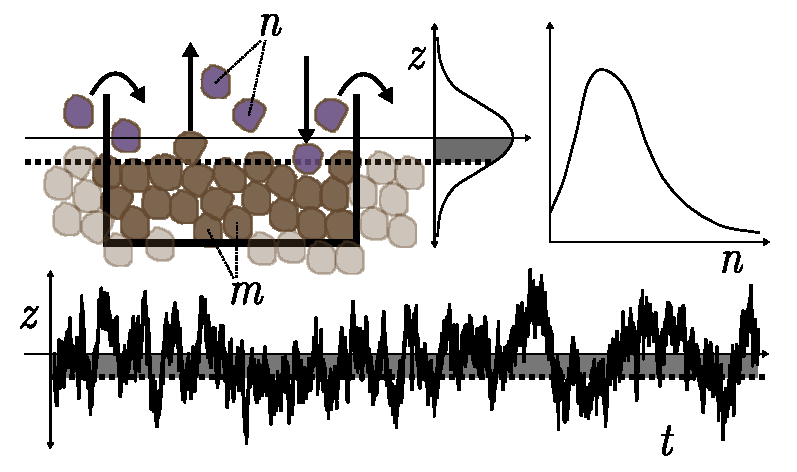
\includegraphics[width=\linewidth,keepaspectratio]{../figures/definition-combo.pdf}
	\vspace{-1.0cm}
	\caption{Definition sketch of a control volume containing $n$ moving grains and $m$ resting grains. Migration, entrainment, and deposition processes are represented by arrows, and the instantaneous bed elevation is depicted by dotted lines. The bed is displayed in a degraded state, where $m<m_0$. The marginal distributions of $n$ and $m$ are indicated in the upper right panel, while the lower panel is a realized time-series of bed elevations computed from $m$ using (\ref{eq:ele}).}
	\label{fig:concept}
	\vspace{-0.75cm}
\end{figure}
%\end{comment}

% describe the set up 
We define a volume of downstream length $L$ that contains some number $n$ of moving particles in the water flow and some number $m$ of stationary particles composing the bed at time $t$ as depicted in figure \ref{fig:concept}.
For simplicity, we consider all particles as approximately spherical with the same diameter $2a$, so their mobility and packing characteristics are similar.
Following \citet{Ancey2008}, we prescribe four events that can occur at any instant to modify the populations $n$ and $m$, and we characterize these events using probabilities per unit time, or rates.
These are: (1) migration of a moving particle into the volume from upstream ($n \rightarrow n+1$); (2) the entrainment (i.e., erosion) of a stationary particle into motion within the volume ($m\rightarrow m-1$ and $n\rightarrow n+1$); (3) the deposition of a moving particle to rest within the volume ($m\rightarrow m+1$ and $n\rightarrow n-1$); and (4) the migration of a moving particle out of the volume to downstream ($n\rightarrow n-1$).
These four events are depicted as arrows in figure \ref{fig:concept}.
As the events occur at random intervals, they set up a joint stochastic evolution of the populations $n$ and $m$ characterized by a joint probability distribution $P(n,m,t)$ having marginals $P(n,t) = \sum_m P(n,m,t)$ and $P(m,t) = \sum_n P(n,m,t)$ for the number of particles in motion and at rest in the volume at $t$.


The populations $n$ and $m$ provide the bulk bedload flux $q_s$ and the local bed elevation $z$.
The mean bedload transport rate is given by $q_s \propto u_s \langle n \rangle$, where $u_s$ is the characteristic velocity of moving bedload and $\langle n \rangle = 
\sum_{n,m}nP(n,m) $ is the mean number of grains in motion \citep[e.g.,][]{Charru2004, Ancey2008, Furbish2012a}.
The bed elevation is related to $m$ though the packing geometry of the bed.
To derive this, we prescribe a mean number of grains at rest $m_0$ and introduce a packing fraction $\phi$ of grains in the bed \citep{Torquato2018}.
Considering a two-dimensional bed \citep[e.g.,][]{Einstein1950, Paintal1971}, the deviation from the mean bed elevation is
\begin{equation} z(m) = \frac{\pi a^2}{\phi L}(m-m_0) = z_1(m-m_0). \label{eq:ele}
\end{equation}
The constant $z_1 = \pi a^2/(\phi L)$ is an important scale of the problem. 
$z_1$ is the magnitude of bed elevation change (in an average sense across the control volume) associated with the addition or removal of a single grain.
We write the rates of the four possible transitions as \citep[e.g.,][]{Ancey2008}:
\begin{align}
 &R_{MI}(n+1,m|n,m) = \nu & \text{migration in}, \label{eq:rate1}\\
 &R_E(n+1,m-1|n,m) =\lambda(m) + \mu(m) n  & \text{entrainment},  \label{eq:rate2}\\
 &R_D(n-1,m+1|n,m) =\sigma(m) n & \text{deposition},\label{eq:rate3}\\
 &R_{MO}(n-1,m|n,m) =\gamma n & \text{migration out\label{eq:rate4}}.
\end{align}
These rates are independent of the past history of the populations and depend only on the current populations $(n,m)$. 
As a result, the system is Markovian \citep[e.g.,][]{Cox1965, VanKampen1992}, meaning time intervals between any two subsequent transitions are exponentially distributed \citep[e.g.,][]{Gillespie2007}.

In (\ref{eq:rate1}-\ref{eq:rate4}), $\nu$ and $\gamma$ are constants characterizing migration rates of individual grains into and out of the volume. 
They lack any dependence on the populations $n$ and $m$.
In contrast, $\lambda(m)$, $\mu(m)$, and $\sigma(m)$, characterizing the entrainment, collective entrainment \citep[e.g.,][]{Ancey2008, Heyman2013, Heyman2014}, and deposition rates of individual grains are considered to depend on $m$.
As is well-known, bed elevation changes modify the likelihood of entrainment and deposition in a negative feedback \citep{Sawai1987, Wong2007}; that is, aggradation increases the likelihood of entrainment, while degradation increases the likelihood of deposition.
\citet{Wong2007} concluded that bed elevation changes induce an exponential variation in entrainment and deposition probabilities, while \citet{Sawai1987} concluded that the variation is linear.
For simplicity, we incorporate the scaling of \citet{Sawai1987} and note its equivalence to the \citet{Wong2007} scaling when bed elevation changes are small.
Because experimental distributions of bed elevations are usually symmetrical, \citep{Wong2007, Singh2009, Martin2014}, we expect the erosion and deposition feedbacks to be anti-symmetrical.
That is, as bed elevation changes drive up (down) erosion rates, so they drive down (up) deposition rates to the same degree.


% set up the m dependence of the rates
Summarizing these ideas, the entrainment and deposition rates can be written $\chi(m) = \chi_0(1\pm z_1 z(m)/(2l)^2)$, where $\chi = \lambda, \mu, \sigma$, and the entrainment parameters take the plus sign, while deposition takes the minus, and we have introduced a length scale $l$.
The variance of bed elevation turns out to be given by $\text{var}(z) = (l / z_1)^2$. Accordingly, $l$ characterizes the range of bed elevation variations, which could be interpreted as an active layer depth \citep[e.g.,][]{Church2017}.
Another perspective is that $l$ is the distance of bed elevation change at which the entrainment and deposition rates are significantly affected.
With these substitutions, the local bed elevation-dependent entrainment and deposition rates (\ref{eq:rate2}-\ref{eq:rate3}) can be written:
\begin{align}
R_E(n+1,m-1|n,m)&=[\lambda_0 + \mu_0 n]\Big[1 + \frac{z_1z(m)}{(2l)^2}\Big], && &\text{entrainment}, \label{eq:rate5}\\
R_D(n-1,m+1|n,m)&=\sigma_0 \Big[1-\frac{z_1z(m)}{(2l)^2}\Big]n, && &\text{deposition}. \label{eq:rate6}
\end{align}
At $z(m)=0$, the rates reduce to those of the \citet{Ancey2008} model.
Away from this elevation, entrainment and deposition are alternatively suppressed and accentuated depending on the sign of $z(m)$.


In terms of the transition rates (\ref{eq:rate1}-\ref{eq:rate6}), we can obtain the Master equation for the probability flow using the forward Kolmogorov equation $\partial P(n,m;t)/\partial t = 
\sum_{n',m'} R(n,m)P(n',m';t)$ \citep[e.g.,][]{Cox1965, Gillespie1992, Ancey2008} as 
\begin{multline}
 \frac{\partial P}{\partial t}(n,m;t) =  
\nu P(n-1,m;t) + 
\{\lambda(m+1) + [n-1]\mu(m+1)\}P(n-1,m+1;t)\\ + 
[n+1]\sigma(m-1)P(n+1,m-1;t) + 
[n+1]\gamma P(n+1,m;t) \\- 
\{ \nu + \lambda(m) + n\mu(m) + n\sigma(m) + n \gamma \}P(n,m;t).
 \label{eq:master}
\end{multline}
The joint probability distribution $P(n,m;t)$ solving this equation will fully characterize the statistics of $n$ and $m$.
We anticipate that solutions will adjust from the initial conditions to a steady-state distribution $P_s(n,m)$, independent of time, if the constant factors in the transition rates are representative of steady bedload transport conditions.
This Master equation describes a two-species stochastic birth-death model \citep[e.g.,][]{Cox1965} of a type well-known in population ecology \citep[e.g.,][]{Pielou1977, Swift2002} and chemical physics \citep[e.g.,][]{Gardiner1983}.
In our context, the two species are the moving and stationary grains in the volume.

\section{Numerical simulations}

Unfortunately, (\ref{eq:master}) does not appear to admit an analytical solution (but see \citet{Swift2002} for a standard method that fails in this case).
The difficulty stems from the product terms between $n$ and $m$.
In response, we resort to numerical methods, simulating (\ref{eq:master}) with the Gillespie algorithm \citep{Gillespie1977, Gillespie1992, Gillespie2007}.
The Gillespie algorithm leverages the defining property of a Markov process: when transition rates do not depend on the past, time intervals between transitions are exponentially distributed \citep[e.g.,][]{Cox1965}.
As a result, to step the Markov process through a single transition, it's enough to draw a random value from the exponential distribution of transition intervals to determine the time of the next transition.
Then drawing another random value to choose the type of transition that occurs using the relative probabilities (\ref{eq:rate1}-\ref{eq:rate6}), the transition can be enacted by shifting $t$, $n$ and $m$ by the appropriate values (i.e., entrainment is $m\rightarrow m-1$ and $n \rightarrow n+1$, and so on).
This procedure can be iterated to form an exact realization of the stochastic process \citep[e.g.,][]{Gillespie2007}.

%\begin{comment}
\begin{wraptable}{l}{0.5\textwidth}
	\caption{Parameters from \citet{Ancey2008} experiments describing the rates of migration in, entrainment, deposition, and migration out when $z(m)=0$. All units are $s^{-1}$ (probability/time). In our model, bed elevation changes modulate these rates in accord with (\ref{eq:rate1}-\ref{eq:rate6}).}\label{tab:anceyparams}
	\begin{tabular}{cccccc} \\ 
		\toprule  
		Flow & $\nu$ & $\lambda_0$ & $\mu_0$ & $\sigma_0$ & $\gamma$ \\
		\midrule
		(a) & 5.45  & 6.59  & 3.74 & 4.67 & 0.77 \\
		\midrule
		(g) & 7.74  & 8.42  & 4.34 & 4.95 & 0.56 \\
		\midrule
		(i) & 15.56 & 22.07 & 3.56 & 4.52 & 0.68 \\
		\midrule
		(l) & 15.52 & 14.64 & 4.32 & 4.77 & 0.48 \\
		\midrule
		(n) & 15.45 & 24.49 & 3.64 & 4.21 & 0.36 \\
		\bottomrule
	\end{tabular}
\end{wraptable} 
%\end{comment}
In this way, we simulated 5 transport conditions with 10 different values of $l$ taken across a range from $l=a$ (a single radius) to $l=10a$ (10 radii).
These values lie in the range exhibited by the majority of available experimental data \citep{Wong2007,Singh2009,Martin2014}.
For the migration, entrainment, and deposition parameters at each flow condition $(\nu, \lambda_0, \mu_0, \sigma_0, \gamma)$, we used values measured by \citet{Ancey2008} in a series of flume experiments.
These are summarized in table \ref{tab:anceyparams}.
Flow conditions are labeled (a), (g), and so on, roughly in order of increasing bedload flux (see \citet{Ancey2008} for more details). 
In all simulations, we take the packing fraction $\phi = 0.6$, a typical value for a pile of spheres \citep[e.g.,][]{Bennett1972}, and set $L = 22.5$cm and $a = 0.3$cm in accord with the \citet{Ancey2008} experiments.
Each simulation was run for $1500$hrs of virtual time, a period selected to ensure convergence of the resting time statistics.

\section{Results}

Our simulations show dynamic time-series of bedload activities and bed elevations (as seen in the lower panel of figure \ref{fig:concept}).
From our chosen initial conditions, all simulations show a rapid attainment of steady-state stochastic dynamics of $n$ and $m$ which support a time-independent joint distribution $P_s(n,m)$. 
We compute this joint distribution by counting occurrences of the states $(n,m)$ in the simulated time series.
From this joint distribution we compute marginals $P(n)$ and $P(m)$ as explained in section \ref{sec:model}.

%\begin{comment}
\begin{wrapfigure}{r}{0.5\textwidth}
	\centering
	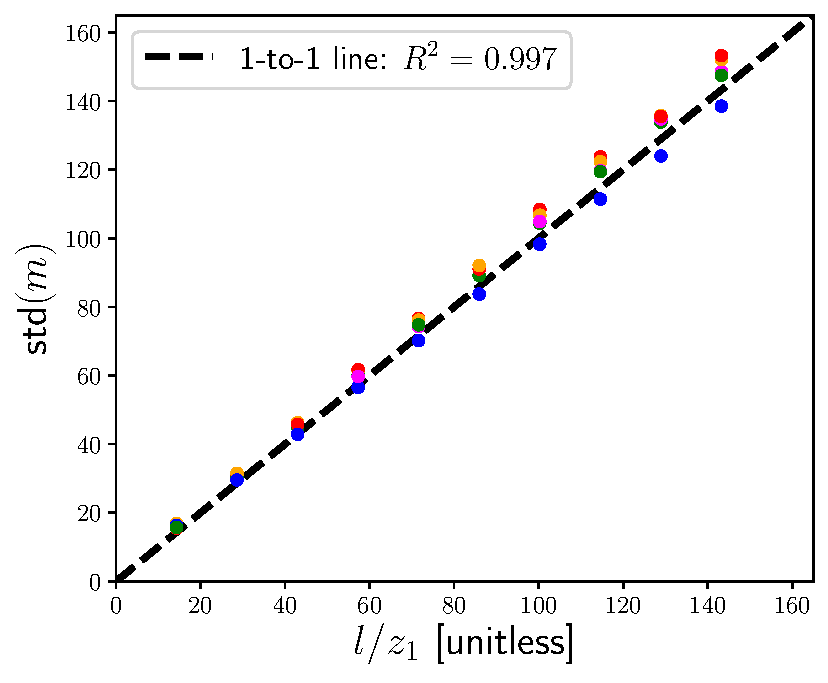
\includegraphics[width=0.5\textwidth,keepaspectratio]{../figures/variance.pdf}
	\caption{Data from all simulations is plotted to show that $l$ controls deviations of bed elevations: $\text{var}(m) = (l/z_1)^2$. }
	\label{fig:var}
\end{wrapfigure}
%\end{comment}
A representative subset of these marginal distributions is displayed in figure \ref{fig:pdfs}.
In their model, \citet{Ancey2008} analytically derived negative binomial distributions for the bedload activity $n$, and this functional form appears preserved through our inclusion of feedbacks between bedload transport and bed elevation changes.
All our computed distributions admit clean negative binomial fits (figure \ref{fig:pdfs}a).
For the bed elevation $m$ (or $z$), our computations show Gaussian distributions (figure \ref{fig:pdfs}b), consistent with our assumptions of a symmetric scaling of erosion and deposition rates with bed elevation changes \citep[e.g.,][]{Wong2007}.


From the marginal distributions, we calculate means and variances of bedload activity ($n$) and bed elevation ($m$).
The mean bed elevation is $m_0$, the parameter in (\ref{eq:ele}). $m$ fluctuates around this value because it sets the equilibrium position of the elevation-related feedbacks within (\ref{eq:ele}).
The variance of $m$ follows $z_1^2 \text{var}(m) = l^2$, as demonstrated in figure \ref{fig:var}, consistent with our interpretation of $l$ as a measure of bed elevation fluctuations.
The variance of $n$ ($\text{var}(n)$), characterizing the magnitude of bedload activity fluctuations, has a more nuanced dependence on the coupling of transport to bed elevation changes.
Generally speaking, our simulations show relatively small $\text{var}(m)$ increases $\text{var}(n)$ from its decoupled value (i.e., its $l\rightarrow \infty$ value), while relatively large $\text{var}(m)$ decreases $\text{var}(n)$ from its decoupled value.
Since $\text{var}(m)$ reflects the coupling between entrainment/deposition rates and the local bed elevation, we see a relatively strong coupling (small $l$) increases bedload fluctuations, while a relatively weak coupling (large $l$) reduces them.
In simple terms, when bed elevation variations are tightly linked to the mobility of surface grains, bedload fluctuations are enhanced.

%\begin{comment}
\begin{figure}
	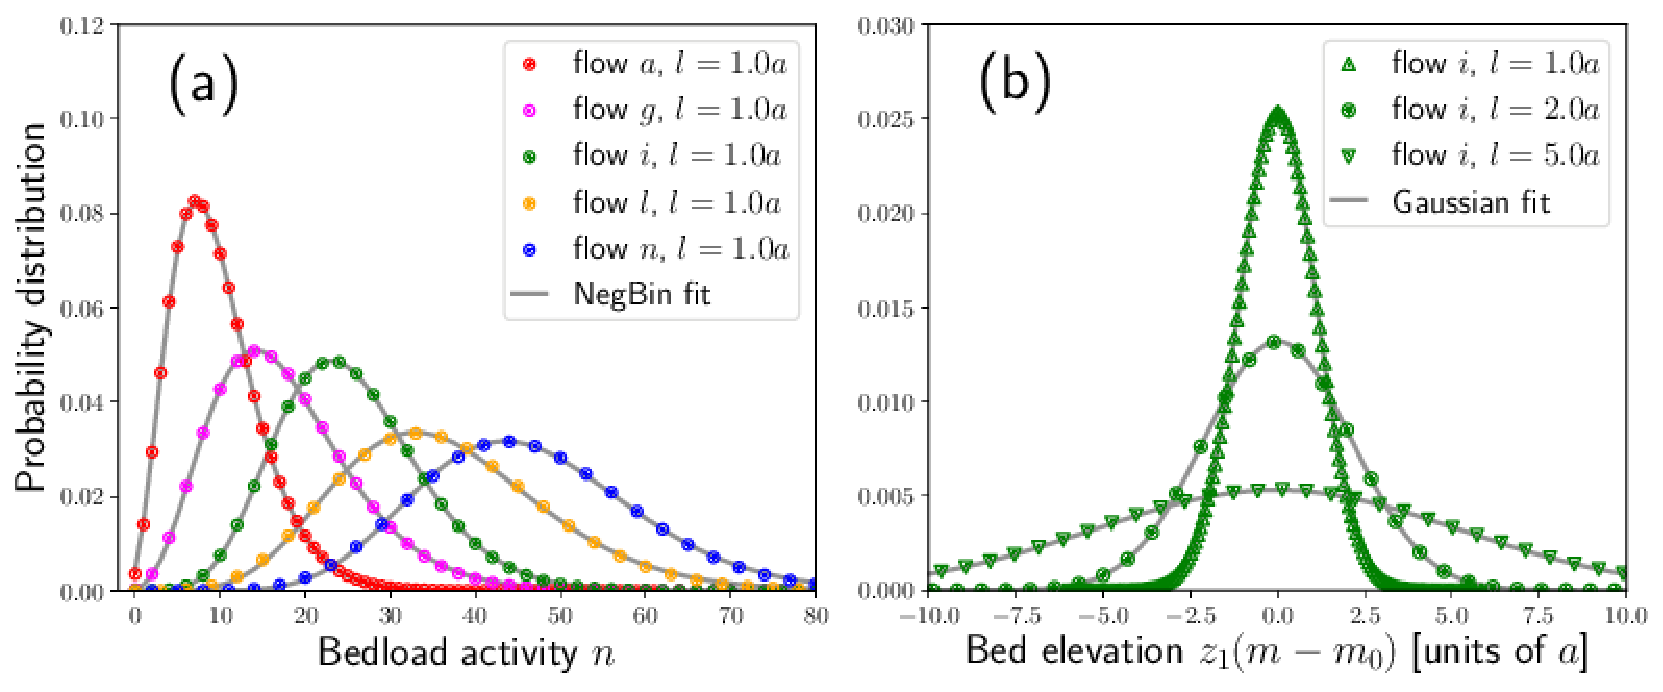
\includegraphics[width=\linewidth,keepaspectratio]{../figures/montage2.pdf}
	\caption{Marginal distributions of $n$ and $m$ for a representative subset of simulations. Some points have been omitted for clarity.}
	\label{fig:pdfs}
\end{figure}
%\end{comment}

%\begin{comment}
\begin{figure}[t!]
	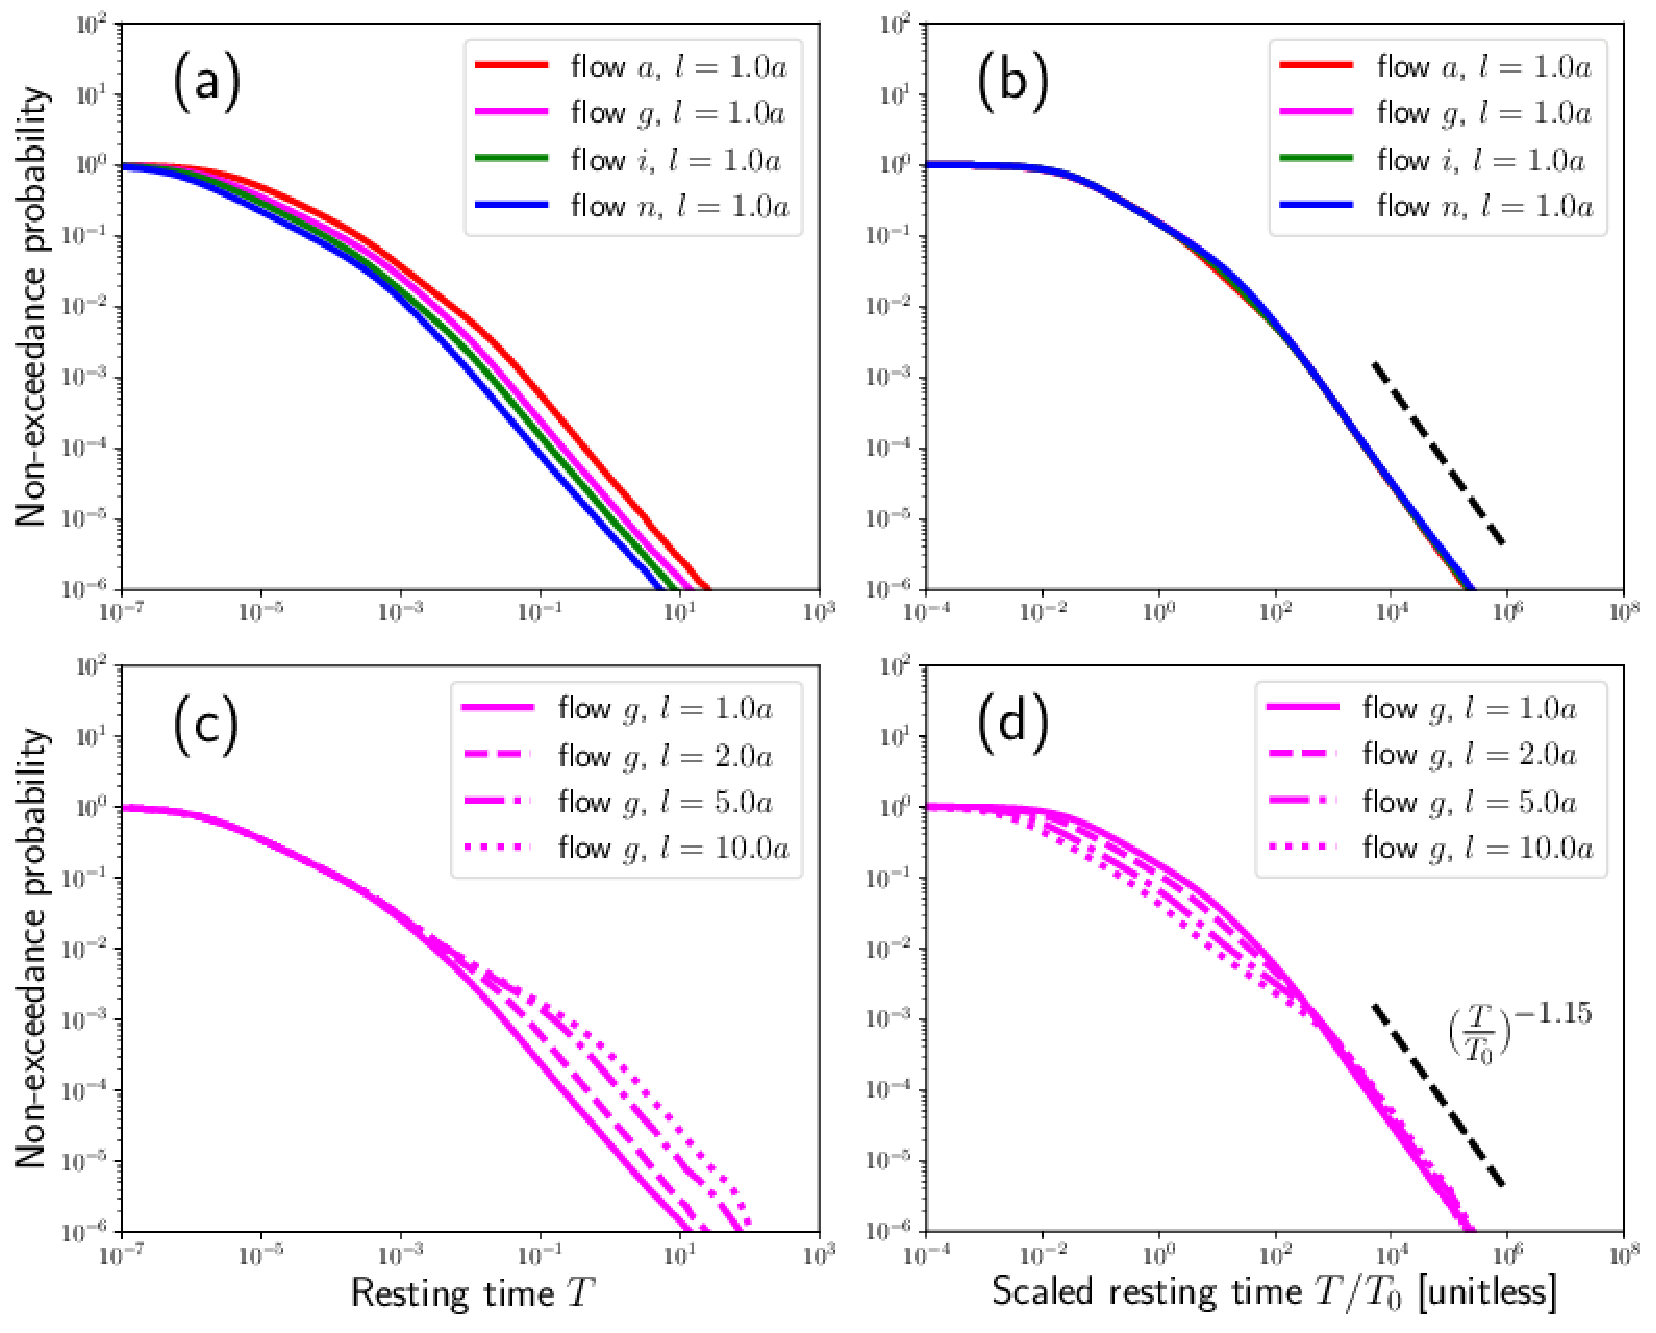
\includegraphics[width=\linewidth,keepaspectratio]{../figures/montage1.pdf}
	\caption{Resting time statistics scale differently with transport conditions and the bed elevation variance. Panel (a) shows differing flow conditions at a fixed $l$ value, while panel (c) shows fixed flow conditions at differing $l$. When scaled by $T_0$ (\ref{eq:time}), both types of difference collapse in the tails of the distributions, as shown in panels (b) and (d). In panels (b) and (d), the black dotted lines indicate a power law decay of the collapsed tails having parameter $\alpha\approx1.18$ .}
	\label{fig:cdfs}
\end{figure}
%\end{comment}
Resting times for sediment undergoing burial are obtained from the time-series of $m$.
Following \citet{Voepel2013} and \citet{Martin2014}, we concentrate on a particular bed elevation $m'$, and find all time intervals separating deposition events at $m=m'$ from erosion events at $m=m'+1$.
These are the return times from above of the sedimentary bed conditional to the elevation $m'$.
Binning these conditional return times (using logarithmically-spaced bins to reduce computational load) and counting the occurrences in each bin, we obtain a non-exceedance distribution of return times $t_r$ held conditional to the elevation $m'$: $P(T>t_r|m')$.
Using the marginal probability distribution of bed elevations $P(m)$, we derive the unconditional non-exceedance distribution of resting times as a sum over all elevations \citep{Yang1971, Nakagawa1980, Voepel2013, Martin2014}:
\begin{equation} P(T>t_r) = \sum_{m'} P(m') P(T>t_r|m') .\end{equation}
Some of these results are displayed in figure \ref{fig:cdfs}.
In contrast to earlier works our analysis does not require an additional binning step over the elevation, since our elevation series is discrete (multiples of $z_1$).
This provides enhanced resolution of the resting time distributions.
Comparing panels \ref{fig:cdfs}(a) and \ref{fig:cdfs}(c) shows the resting time distributions scale with the intensity of bedload transport and the standard deviation of bed elevations ($l$) in different ways.
However, as shown in panels \ref{fig:cdfs}(b) and \ref{fig:cdfs}(d), a characteristic timescale $T_0$ is found to collapse away both of these types of differences.
We obtain $T_0$ heuristically by finding a characteristic speed of bed elevation change.
Formally, the mean erosion rate is $E = \sum_{n,m}R_E(n+1,m-1|n,m)P_s(n,m)$.
This is the mean number of grains leaving the bed per unit time.
Since the removal of a single grain changes the bed elevation by $z_1$, bed elevations change with a characteristic speed $z_1 E$.
Since the range of elevation deviations is $l$, the time required for the bed to shift through this characteristic distance is
\begin{equation} T_0 = \frac{l}{z_1 E}.\label{eq:time}\end{equation}
When scaling the resting time by this $T_0$, we obtain the collapse shown in figure \ref{fig:cdfs}.
Using the log-likelihood estimation technique described by \citet{Newman2005}, we estimate the scaled resting time non-exceedance distributions decay as a heavy-tailed power law with parameter $\alpha = 1.18 \pm 0.32$ for all return times satisfying $T/T_0 > 10^3$.
These distributions are sufficiently heavy-tailed to violate the central limit theorem and drive anomalous super-diffusion of bedload, a result which supports the earlier conclusions of \citep{Martin2014}.

\section{Discussion}

% A) discuss the historical context and the classic related work
\citet{Einstein1937} developed the first model of individual bedload motions and bedload diffusion, and his ideas can be viewed as the historical nexus of an entire paradigm of research that extends into the present day \citep[e.g.,][]{Hubbell1964, Nakagawa1976,Hassan1991,Ancey2008, Wu2019}.
Works in this paradigm attempt to understand properties of bedload transport from applying a stochastic concept of individual sediment motions.
With some exceptions \citep[e.g.,][]{Yang1971,Nakagawa1980,Pelosi2016,Wu2019}, existing descriptions are spatially one-dimensional, concentrating on the motion of grains in the downstream direction without including the vertical dimension wherein local bed elevation changes imply sediment burial \citep[e.g.,][]{Voepel2013,Martin2014} and modify the mobility of surface grains \citep[e.g.,][]{Yang1971,Nakagawa1980}.

% B) Discuss what you did, what its limitations are, and how your it links to the historical context
Our model builds upon several earlier works \citep[e.g.,][]{Ancey2008,Martin2014} to include this vertical dimension and provide a joint description of bedload transport and bed elevation changes.
We find negative binomial distributions of bedload activity and normal distributions of bed elevations, reproducing a wide set of experimental findings \citep{Ancey2008, Heyman2016, Wong2007, Singh2009, Martin2014}.
More importantly, we interpret resting times of sediment undergoing burial as return times from above in the bed elevation time series \citep[e.g.,][]{Voepel2013,Martin2014}, and predict the form and characteristics of this distribution.
Of course, modeling complex geophysical phenomena (such as expressions of coupled fluid and granular phases) necessitates simplifying assumptions \citep[e.g.,][]{Larsen2016}, and our work is no exception.
We believe the key limitations of our work are (1) our assumption that local (as opposed to non-local) deviations in bed elevation are the dominant control on the mobility of grains; and (2) those assumptions inherited from the underlying bedload transport model of \citet{Ancey2008}, which essentially incorporates the earlier assumptions of \citet{Einstein1950} into a stochastic framework.
The first assumption can be somewhat justified under conditions in which the formation of organized bed structures is not favored \citep[e.g.,][]{Hassan2008}, while the second has been discussed in earlier works and appears justified in near-threshold transport conditions when the intermittent aspect of bedload transport is emphasized \citep[e.g.,][]{Ancey2008,Heyman2014} whenever organized bed structures are not present \citep[e.g.,][]{Dhont2018}.

The joint description (\ref{eq:master}) reproduces earlier descriptions of bedload activities by \citet{Ancey2008} and bed elevations by \citet{Martin2014} in simplified limits.
The \citet{Ancey2008} bedload model is obtained when bed elevation fluctuations $\delta m$ are considered small: $m \approx m_0$.
Taking account of this change in (\ref{eq:master}) obtains the master equation of \citet{Ancey2008} for the bedload activity distribution $P(n,t)$.
Hence the differences between our bedload activity statistics and those of the \citet{Ancey2008} model are induced by bed elevation fluctuations.
When relatively large bed elevation fluctuations are possible (i.e., $l$ is large), bed elevation changes act to buffer bedload activity fluctuations.
In contrast, when bed elevation changes are tightly linked to the mobility of moving and stationary grains (i.e., $l$ is small), bed elevation changes enhance bedload fluctuations.
We hypothesize this enhancement/suppression of bedload fluctuations is primarily due to the collective entrainment term in (\ref{eq:rate6}), since the \citet{Ancey2008} variance is most sensitive to the collective entrainment process.
However, more research will be required to clarify the linkage between bed elevation changes and bedload fluctuations.
Given recent observations of sudden local elevation changes being induced by avalanches on the downstream face of bars \citep{Dhont2018}, we identify the interplay between collective motions of bedload and bed elevation changes as an emerging research theme, and we suggest our joint description may hint toward a modeling framework to address these issues.

The \citet{Martin2014} bed elevation model based upon the Ornstein-Uhlenbeck (OU) process is obtained in the converse limit when bedload activity fluctuations $\delta n$ are small: $n \approx \langle n \rangle$.
In this case, neglecting the migration terms and identifying the mean entrainment and deposition rates as $E =\lambda_0 + \mu_0 \langle n \rangle$ and $D = \sigma_0 \langle n \rangle$ before using the steady-state transport condition $E=D$ \citep[e.g.,][]{Einstein1950} gives
\begin{equation} \frac{\partial}{\partial t}P(m,t) =  E \Big\{ \Big[1 +\Big(\frac{z_1}{2 l}\Big)^2m\Big]P(m+1,t) +  \Big[1 -\Big(\frac{z_1}{2 l}\Big)^2m\Big]P(m-1,t) - 2P(m,t)\Big\}, \label{eq:ou}\end{equation}
This is a discrete state analogue of the OU process \citet{Martin2014} used to model bed elevation changes, and it provides excellent correspondence to the bed elevation statistics and resting time distributions computed from our joint model.
Our resting time distributions of sediment undergoing burial essentially correspond with those of \citet{Martin2014} given our computational uncertainty.
These authors proposed $\alpha \approx 1 $ from a continuum analogue of (\ref{eq:ou}).
Incidentally, they scale resting times by an "activity parameter" $1/a$ which is equivalent to $1/(2E)$ in our notation.
Our work suggests the incomplete collapse displayed by \citet{Martin2014} may be corrected by including a bed elevation variance factor in their scaling as in (\ref{eq:time}), further justifying the correspondence of our model to (\ref{eq:ou}).
In fact, we note $T_0$ is the autocorrelation time of the limiting OU process (\ref{eq:time}) \citep[e.g.,][]{Gardiner1983}.

In light of the coupling between elevation fluctuations and the entrainment/deposition rates in (\ref{eq:master}), and the non-negligible elevation fluctuations our model produces (figure \ref{fig:pdfs}b), this correspondence to \citet{Martin2014} is initially surprising.
However, we can understand it through the lens of "fast" and "slow" stochastic variables advanced by \citet{Haken1983}.
Since appreciable bed elevation changes are the compound result of many bedload entrainment or deposition events ($O(l/z_1)$ of them), bed elevation fluctuations persist for a typical timescale which is much longer than the timescale of bedload activity flucutations, so $n$ is a "fast" variable while $m$ is a "slow" one.
This statement could be formalized by comparing the autocorrelation times of $n$ and $m$ \citep[e.g.,][]{Gardiner1983}.
Accordingly, the value of $m$ does not change appreciably during the period of time required for $n$ to vary through a wide range, meaning the slow variable $m$ is influenced by many $n$ values during the course of its incremental evolution, justifying the mean-field limit (\ref{eq:ou}) equivalent to \citet{Martin2014}.
This is a so-called adiabatic slaving principle, whereby fast stochastic variables are coordinated to slow ones but not the converse.
Hence (\ref{eq:ou}) is justified from a more rigorous adiabatic approximation of (\ref{eq:master}) based on integrating out the fast variable $n$ \citep[e.g.,][]{Haken1983,Gardiner1983}, and not only by an ad hoc mean-field limit.
We believe such ideas may find widespread application to future river science considerations.
Indeed, rivers display a wide set of temporally evolving attributes, exhibiting apparent randomness on disparate scales \citep{Chartrand2019}, including hydraulic flow \citep[e.g.,][]{Ferrer-Boix2015}, morphological structure \citep[e.g.,][]{Dhont2018}, and sediment supply regime \citep[e.g.,][]{Elgueta-Astaburuaga2019}.
This increasing realization has encouraged investigators to approach river science problems from a stochastic physics standpoint, driving a contemporary increase in the popularity of this approach \citep[e.g][]{Ancey2008,Furbish2012}.
In the present context, we have provided evidence that simpler one-dimensional stochastic models \citep[e.g.,][]{Martin2014} can aptly describe more complex geophysical phenomena when a scale mismatch is present in their coupled components.


% E) discuss your key conclusions on resting time distributions and bedload diffusion / discuss relationship to field studies and laboratory experiments
The computed resting time distributions (figure \ref{fig:cdfs}) provide several implications for bedload diffusion.
Our simulations show asymptotic power law tails with parameter $\alpha = 1.18 \pm 0.32$ after scaling by $T_0$ related to the characteristic speed of bed elevation changes.
For a general power law, if $\alpha>1$, neither the mean or variance of the resting time will converge, while if $1<\alpha <2$, the mean will converge while the variance will not \citep[e.g.,][]{Bradley2017}.
Within our computational uncertainty stemming from the finite duration of our simulations and the log-likelihood estimation of $\alpha$ \citep[e.g.,][]{Newman2005}, we are unable to conclude whether the mean resting time will diverge, but we can conclude the variance will diverge.
According to \citet{Weeks1998}, if the step length distribution has a light tail \citep[e.g.,][]{Hassan2013}, our computed power-law resting times are sufficiently heavy-tailed to imply diffusion scaling as either $\sigma_x^2 \propto t^{3-\alpha} \approx t^{\{1.82 \pm 0.32 \}}$ or $\sigma_x^2 \propto t^{2\alpha} \approx t^{\{3.64\pm 0.45\}}$ at asymptotically large times.
In either case, the process of sediment burial induces an extreme super-diffusion of bedload: at long timescales, some grains will continue to transport downstream in alternate motion-rest sequences while others will become trapped under the bed for relatively long periods of time, driving a rapid spreading of the population.
In relation to solid contaminant export from river channels \citep[e.g.,][]{Malmon2005}, long-time super-diffusion implies contaminants will eventually dilute over a relatively vast region. However, heavy-tailed resting times mean total evacuation could take an exceedingly long time.

% F) Discuss scope for extension and shortcomings
Finally, we propose a possible extension of the joint model (\ref{eq:master}) by following its linkage to \citet{Ancey2008} and follow-ups \citep[e.g.,][]{Ancey2014a, Heyman2014, Heyman2015}.
These works are based on chaining many \citet{Ancey2008} single-cell models together along a line, with migration out of one cell being migration into another.
In this way, they provide a framework to study spatial correlations in bedload transport \citep[e.g.,][]{Heyman2014,Heyman2015}.
Similar approaches have been used to formulate reaction-diffusion and flow problems in stochastic physics \citep[e.g.,][]{Gardiner1983}. 
One can imagine using the model (\ref{eq:master}) in the same way, chaining an array of volumes (as in figure \ref{fig:concept}) together along a line to generate a fluvial morphodynamics model ultimately rooted in a stochastic concept of individual motions \citep[e.g.,][]{Einstein1937}.
Such a model could provide spatial correlations in bed elevation changes and bedload transport while taking account of their inherent granularity.
Given the increasing realization that granular physics phenomena initiated by individual grains, such as avalanches and jamming, play a non-negligible role in fluvial processes \citep[e.g.,][]{Saletti2016,Dhont2018}, we speculate such a model, if suitably extended, might provide unique traction on future research problems centered around processes initiated by individual grains.


\section{Conclusion}

We have developed a joint stochastic model of bedload transport and bed elevation changes based upon the motions of individual grains, fusing earlier works in the research paradigm of \citet{Einstein1937}.
This is a two-population stochastic birth-death process of a type often encountered in mathematical ecology \citep[e.g.,][]{Pielou1977} and chemical physics \citep[e.g.,][]{Gardiner1983}, and it reproduces empirical expectations for Gaussian bed elevation and negative binomial bedload activity distributions \citep[e.g.,][]{Wong2007,Ancey2008}.
Interpreting resting times of sediment undergoing burial as return times from above in the bed elevation time series \citep[e.g.,][]{Voepel2013}, we predict asymptotic heavy-tailed power-law resting times with parameter $\alpha = 1.18 \pm 0.32$, corroborating the results of \citet{Martin2014}.
These distributions imply sediment burial will induce bedload super-diffusion at long timescales \citep[e.g.,][]{Phillips2013}.
Finally, this work draws some concepts from the stochastic physics literature into river science for the first time, and it points out several difficult problems for future research.
The limit of our description to the model of \citet{Martin2014} provides a geophysical example of Haken's slaving principle concerning the interaction of fast and slow stochastic variables \citep{Haken1983}, and its comparison to \citet{Ancey2008} suggests a nuanced linkage between collective transport and bed elevation changes which requires further study.

\acknowledgments
The simulation code is freely available at
\sloppy
\url{https://drive.google.com/file/d/1bWEX_ZHlcGRKCxtRIadnSbhh4EpQlsoh/view?usp=sharing}.
This research was supported by an NSERC Discovery Grant to M. Hassan.
We would like to thank Shawn Chartrand and Conor McDowell for helpful discussions.

\bibliography{biblio}

\end{document}



